\chapter{Scaling Laws and Model Behavior}\index{scaling laws}\index{model behavior}
\label{chap:scaling_laws}

\noindent
As LLMs\index{LLM|see {Large Language Model}}\index{Large Language Model} grow larger, surprising empirical regularities---often termed ``scaling laws''---begin to emerge. This chapter explores how model performance\index{model!performance}, data requirements\index{data!requirements}, and computational costs\index{computational costs} scale together, and why overparameterized networks\index{overparameterization} can sometimes generalize better than smaller ones.

\section{Empirical Scaling Laws}\index{scaling laws!empirical}
\label{sec:empirical_scaling}

\subsection{Power Law Relationships}\index{power law}
\noindent
Research has identified several key power-law relationships in LLM training. These laws suggest that increasing the number of parameters in a model, or the amount of data it is trained on, often leads to predictable improvements in performance, but that these improvements follow a power-law distribution. In simpler terms, each additional parameter or data point contributes less than the previous one. This implies the existence of a point of diminishing returns. Specifically, the relationship between model size, dataset size, and the model's loss (a measure of error) can often be approximated by a power law, as shown below:

\begin{equation}\label{eq:loss_scaling}
\text{Loss} \approx \left(\frac{N_{\text{params}}}{N_{\text{critical}}}\right)^{-\alpha} + \left(\frac{N_{\text{data}}}{D_{\text{critical}}}\right)^{-\beta} + L_{\text{irreducible}}
\end{equation}

where:
\begin{itemize}[noitemsep]
    \item \(N_\text{params}\)\index{parameters!number of}: Number of model parameters - essentially the size of the model.
    \item \(N_\text{data}\)\index{data!size}: Training dataset size - the amount of data used to train the model.
    \item \(\alpha, \beta\): Empirically observed scaling exponents - these values determine the steepness of the power-law curve. They are typically found to be between 0.05 and 0.1, with both being less than 1, according to Kaplan's 2020 paper.
    \item \(L_\text{irreducible}\): Irreducible loss component - the baseline error that cannot be reduced by simply increasing model size or data. This represents the inherent noise or randomness in the data or task.
    \item \(N_\text{critical}\), \(D_\text{critical}\): These are constants that represent a critical scale for the number of parameters and data size, respectively. These are the points at which the model starts to significantly benefit from increased size or data.
\end{itemize}

This equation implies that increasing either the number of parameters or the data size will decrease the loss, but with diminishing returns. The irreducible loss represents a fundamental limit on the model's performance.

\subsection{Chinchilla Scaling}\index{Chinchilla scaling}
\noindent
The Chinchilla paper~\cite{hoffmann2022training} established optimal compute-efficient scaling ratios:

\begin{figure}[ht]
    \centering
    \begin{subfigure}[b]{0.40\textwidth}
        \centering
        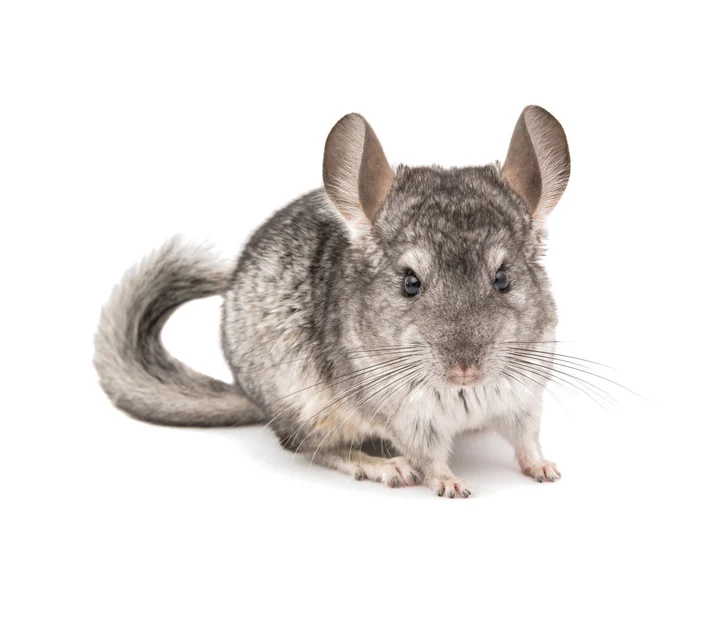
\includegraphics[width=\textwidth]{images/chinchilla.png}
        \caption{Hi! I am Chinchilla. I scale your laws.}
        \label{fig:chinchilla_scaling}
    \end{subfigure}
    \hfill
    \begin{subfigure}[b]{0.52\textwidth}
        \centering
        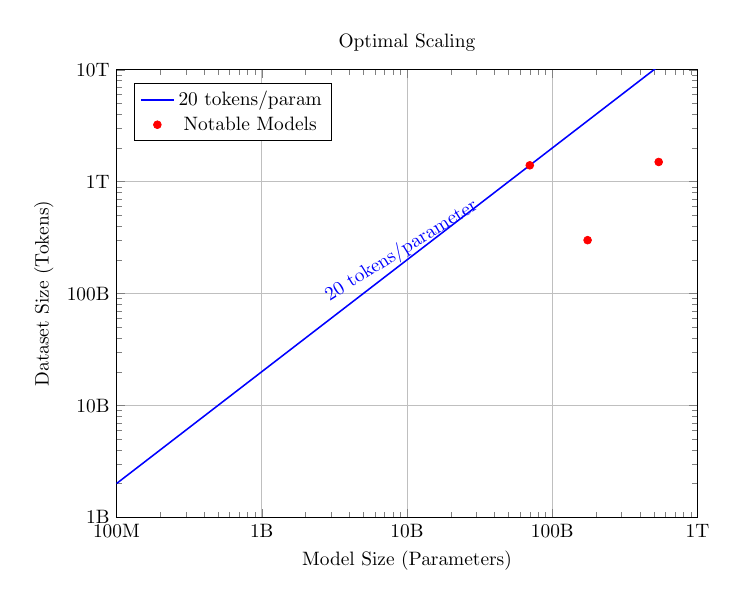
\begin{tikzpicture}[scale=0.7]
            % Set up the axes
            \begin{axis}[
                width=\textwidth,
                height=0.8\textwidth,
                xlabel={Model Size (Parameters)},
                ylabel={Dataset Size (Tokens)},
                xmode=log,
                ymode=log,
                grid=major,
                xmin=1e8, xmax=1e12,
                ymin=1e9, ymax=1e13,
                xtick={1e8,1e9,1e10,1e11,1e12},
                ytick={1e9,1e10,1e11,1e12,1e13},
                xticklabels={100M,1B,10B,100B,1T},
                yticklabels={1B,10B,100B,1T,10T},
                legend pos=north west,
                title={Optimal Scaling}
            ]
            
            % Plot the optimal scaling line (20 tokens per parameter)
            \addplot[thick,blue] coordinates {
                (1e8, 2e9)
                (1e9, 2e10)
                (1e10, 2e11)
                (1e11, 2e12)
                (1e12, 2e13)
            };
            
            % Add some example models as points
            \addplot[only marks,mark=*,red] coordinates {
                (175e9, 300e9)  % GPT-3
                (70e9, 1.4e12)  % Chinchilla
                (540e9, 1.5e12) % PaLM
            };
            
            % Add legend
            \legend{20 tokens/param, Notable Models}
            
            % Add annotation for the optimal ratio
            \node[rotate=32,blue, yshift=5.4] at (axis cs:1e10,2e11) 
                {20 tokens/parameter};
                
        \end{axis}
        \end{tikzpicture}
        \caption{Visualization of the optimal ratio of 20 tokens per parameter (blue line) with notable models (red dots) plotted against their parameter counts and training dataset sizes.}
        \label{fig:chinchilla_scaling_plot}
    \end{subfigure}
    \caption{Chinchilla scaling laws demonstrating the optimal relationship between model size, dataset size, and compute budget.}
    \label{fig:chinchilla_combined}
\end{figure}


\begin{itemize}
    \item \textbf{Parameters to Data Ratio:}\index{parameters!to data ratio} Approximately 20 tokens per parameter
    \item \textbf{Compute-Optimal Training:}\index{compute-optimal training} Balancing model size with dataset size
\end{itemize}

The implication of Chinchilla scaling is that many large language models could be made smaller and trained on more data, leading to similar or better performance while using less compute.

\section{Resource Requirements}\index{resource requirements}
\label{sec:resource_requirements}

Scaling up LLMs has significant implications for the computational resources required. Understanding these resource requirements is crucial for planning and budgeting for model training and deployment.

\subsection{Computational Scaling}\index{computational scaling}
\noindent
Training costs scale predictably with model size and dataset size. The primary computational cost comes from the number of floating-point operations (FLOPs) required during training. A rough estimate of the FLOPs required for training can be approximated by:

\begin{equation}\label{eq:compute_scaling}
\text{FLOPs}_\text{training} \approx 6ND
\end{equation}
where:
\begin{itemize}[noitemsep]
    \item \(N\): Number of parameters in the model.
    \item \(D\): Dataset size in tokens.
\end{itemize}

This formula considers both the forward and backward passes during training. It shows that the computational cost scales linearly with both the model size and the dataset size. This means that doubling either the number of parameters or the number of tokens in the dataset will approximately double the number of FLOPs required for training.  It's worth noting that this is a simplified model, and in practice, factors like model architecture, batch size, and hardware can influence the exact computational cost.

\subsection{Memory Requirements}\index{memory requirements}
\noindent
Memory usage is another critical constraint when training LLMs. The memory required can be broken down into several key components:

\begin{itemize}[noitemsep]
    \item \textbf{Model Parameters:}\index{parameters!memory} \(M_\text{params} = 4N\) bytes (assuming 32-bit floating-point precision, or 4 bytes per parameter). This is the memory needed to store the model's weights.
    \item \textbf{Optimizer States:}\index{optimizer states} \(M_\text{opt} = 8N\) bytes for optimizers like Adam, which maintain two moments (mean and variance) per parameter. Other optimizers may have different memory requirements.
    \item \textbf{Activations:}\index{activations} \(M_\text{act} \approx \mathcal{O}(B \sqrt{N})\) for batch size \(B\). The memory required to store activations (intermediate outputs of each layer) depends on the batch size and the model's architecture. This scaling is a simplified approximation and can vary significantly depending on the model's depth and layer widths. The memory required for activations is often the largest component, especially during training.
    \item \textbf{Gradients:}  \(M_\text{grad} = 4N\) bytes, similar to the model parameters, as gradients need to be computed and stored for each parameter during backpropagation.
    \item \textbf{Forward Activations (for recomputation):} In some cases, especially for very large models, activations from the forward pass are recomputed during the backward pass to save memory. This reduces the memory footprint but increases computation time.
\end{itemize}

These memory components can add up quickly, especially for large models and batch sizes, often exceeding the memory capacity of a single GPU. Techniques like model parallelism and gradient checkpointing are often employed to distribute the memory requirements across multiple devices or to trade off computation for memory.

\section{Performance Scaling}\index{performance scaling}
\label{sec:performance_scaling}

The ultimate goal of scaling up LLMs is to improve their performance on various tasks. Understanding how performance scales with model size, data, and compute is essential for guiding research and development efforts.

\subsection{Task-Specific Scaling}\index{task-specific scaling}
\noindent
Different tasks exhibit varying scaling behaviors. Some tasks show steady improvement with scale, while others may plateau or even degrade. Here's a breakdown:

\begin{itemize}[noitemsep]
    \item \textbf{Language Modeling:}\index{language modeling!scaling}  Language modeling perplexity (a measure of how well the model predicts the next word) tends to show smooth, predictable power-law scaling with both model size and dataset size. This means that larger models trained on more data consistently perform better at language modeling.
    \item \textbf{Reasoning Tasks:}\index{reasoning tasks}  Performance on reasoning tasks (e.g., commonsense reasoning, arithmetic reasoning) often exhibits more complex scaling behavior. There can be sharp transitions or "phase changes" where performance suddenly improves at certain scales, suggesting the emergence of new capabilities.
    \item \textbf{Few-Shot Learning:}\index{few-shot learning}  Few-shot learning, the ability to learn from just a few examples, often shows dramatic improvements with scale. Larger models are significantly better at learning from limited examples, sometimes achieving impressive performance with just a handful of demonstrations. This was one of the key findings of the GPT-3 paper~\cite{brown2020language}, which showed that large language models could perform a wide variety of tasks with little to no task-specific training data.
    \item \textbf{Other downstream tasks:} The scaling behavior on other tasks (e.g., translation, question answering, summarization) can vary. Some tasks show consistent improvements with scale, while others may reach a point of diminishing returns sooner.
\end{itemize}

\subsection{Scaling Plateaus}\index{scaling plateaus}
\noindent
Despite the benefits of scaling, models eventually hit diminishing returns. This can be due to several factors:

\begin{itemize}[noitemsep]
    \item \textbf{Dataset Exhaustion}\index{dataset exhaustion}:  The model may have seen most of the useful information in the available training data. This is particularly relevant for specialized domains where data is limited. Simply adding more data of similar quality may not lead to significant improvements.
    \item \textbf{Task Complexity Limits}\index{task complexity}:  The inherent complexity of the task may impose a fundamental limit on achievable performance, regardless of model size or data. Some tasks may be too difficult to learn perfectly from the available data, even with very large models.
    \item \textbf{Architectural Bottlenecks}\index{architectural bottlenecks}:  The model's architecture itself may become a limiting factor. For example, increasing the number of layers in a Transformer model beyond a certain point can lead to training instability or diminishing returns.
    \item \textbf{Optimization Challenges}: Training very large models can be challenging due to issues like vanishing or exploding gradients, difficulty in finding good optima, and increased sensitivity to hyperparameters.
\end{itemize}

Identifying and overcoming these scaling plateaus is an active area of research in the field of large language models.

\section{Theoretical Understanding}\index{theoretical understanding}
\label{sec:theoretical_understanding}

While empirical scaling laws provide valuable insights, a deeper theoretical understanding is necessary to fully explain these phenomena and guide future research.

\subsection{Double Descent Phenomenon}\index{double descent}
\noindent
The double descent phenomenon is a surprising observation in deep learning that challenges classical statistical learning theory. It describes a situation where increasing model complexity beyond a certain point (the "interpolation threshold") can lead to *improved* generalization performance, contrary to the traditional U-shaped bias-variance trade-off curve.

\begin{itemize}[noitemsep]
    \item \textbf{Classical Regime:}\index{classical regime}  In the classical regime (underparameterized models), the relationship between model size and test error follows the traditional U-shaped curve. Increasing model size initially reduces test error, but after a certain point, it leads to overfitting and increased test error.
    \item \textbf{Modern Regime:}\index{modern regime}  In the modern, overparameterized regime, as model size continues to increase beyond the interpolation threshold (where the model can perfectly fit the training data), test error can decrease again, leading to a second descent. This is known as the "double descent" phenomenon.
    \item \textbf{Scale Effects:}\index{scale effects}  The double descent curve can shift and change shape with scale. In particular, the peak in test error at the interpolation threshold tends to become less pronounced as the overall scale of the model and dataset increases. In some cases, the peak may disappear entirely, leading to a monotonically decreasing relationship between model size and test error. This is known as the "monotonic scaling" regime and is often observed in large language models.
\end{itemize}

Several hypotheses have been proposed to explain double descent, including the role of implicit regularization in overparameterized models, the effect of stochastic gradient descent on finding good solutions, and the geometry of the loss landscape.

\subsection{Neural Scaling Laws}\index{neural scaling laws}
\noindent
Several theoretical frameworks have been proposed to explain the observed scaling laws:

\begin{itemize}[noitemsep]
    \item \textbf{Information Theoretic Bounds}\index{information theory}:  Information theory provides fundamental limits on how well a model can learn from data. These bounds can be used to derive scaling laws that relate model size, dataset size, and performance. For example, the mutual information between the input and output of a model can be used to bound its generalization error.
    \item \textbf{Statistical Learning Theory}\index{statistical learning theory}:  Classical statistical learning theory concepts like VC dimension and Rademacher complexity can be extended to analyze the generalization performance of deep neural networks. These tools can provide insights into how model capacity and dataset size affect generalization, but they often make simplifying assumptions that may not hold for large, overparameterized models.
    \item \textbf{Effective Dimension}\index{effective dimension}:  The concept of effective dimension tries to capture the true complexity of a model, taking into account the fact that overparameterized models may not use all their parameters effectively. The effective dimension can be used to derive scaling laws that are more accurate than those based on the raw number of parameters.  For instance, a model with a billion parameters might only effectively use a fraction of them during inference or training due to factors like redundancy or implicit regularization. The effective dimension tries to quantify this actual utilized capacity, which might scale differently than the total parameter count.
\end{itemize}

These theoretical approaches provide valuable insights, but a complete and universally accepted theory of neural scaling laws remains an open challenge.

\section{Practical Implications}\index{practical implications}
\label{sec:practical_implications}

Understanding scaling laws has significant practical implications for training and deploying LLMs.

\subsection{Training Strategy Optimization}\index{training strategy}
\noindent
Scaling laws can inform several aspects of training strategy:

\begin{itemize}[noitemsep]
    \item \textbf{Model Size Selection}\index{model size selection}:  Scaling laws can help determine the appropriate model size for a given task and compute budget. For example, if a certain level of performance is required, scaling laws can be used to estimate the minimum model size needed to achieve that performance.
    \item \textbf{Dataset Requirements}\index{dataset requirements}:  Scaling laws can guide the collection and curation of training data. They can help estimate the amount of data needed to achieve a desired level of performance with a given model size. Furthermore, based on the Chinchilla findings, a ratio of approximately 20 tokens per parameter should be targeted for compute-optimal training.
    \item \textbf{Compute Budget Allocation}\index{compute budget}:  Scaling laws can inform the allocation of compute resources between model size and training time. They can help determine the optimal trade-off between training a larger model for fewer steps and training a smaller model for more steps. For example, given a fixed compute budget, scaling laws can help determine whether it's better to train a larger model for a shorter time or a smaller model for a longer time.
    \item \textbf{Hyperparameter Tuning}: Scaling laws can also guide hyperparameter tuning. For example, they can suggest how learning rates should be adjusted as model size or dataset size changes.
\end{itemize}

\subsection{Infrastructure Planning}\index{infrastructure planning}
\noindent
Scaling laws have implications for long-term infrastructure planning:

\begin{itemize}[noitemsep]
    \item \textbf{Hardware Requirements}\index{hardware requirements}:  Scaling laws can inform decisions about hardware procurement, such as the number and type of GPUs or TPUs needed to train and deploy large models. They can help estimate the memory and compute requirements for future models.
    \item \textbf{Storage Planning}\index{storage planning}:  As model and dataset sizes grow, storage becomes a significant consideration. Scaling laws can help estimate future storage needs for both training data and model checkpoints.
    \item \textbf{Network Architecture}\index{network architecture}:  Training large models often requires distributed training across multiple devices or machines. Scaling laws can inform the design of the network architecture, such as the bandwidth and latency requirements for inter-device communication.
\end{itemize}

\section{Future Directions}\index{future directions}
\label{sec:future_directions}

Research on scaling laws is an active and rapidly evolving field.

\subsection{Open Questions}\index{open questions}
\noindent
Several key areas require further investigation:
\begin{itemize}[noitemsep]
    \item \textbf{Fundamental Limits}\index{fundamental limits}:  A deeper understanding of the fundamental limits of scaling is needed. What are the theoretical limits on how well a model can perform, given unlimited data and compute? Are there fundamental limits to what can be learned from language data alone?
    \item \textbf{Architecture-Specific Laws}\index{architecture-specific laws}:  Most existing scaling laws have been derived for Transformer-based models. More research is needed to understand how scaling laws vary across different architectures, such as recurrent or convolutional networks.
    \item \textbf{Task Transfer Effects}\index{task transfer}:  How does scaling on one task affect performance on other tasks? Can we develop scaling laws that predict cross-task transfer learning performance? Understanding how performance on one task scales with performance on other tasks is crucial for developing general-purpose AI systems.
\end{itemize}

\subsection{Emerging Trends}\index{emerging trends}
\noindent
New directions in scaling research are emerging:

\begin{itemize}
    \item \textbf{Mixture-of-Experts Scaling}\index{Mixture-of-Experts!scaling}:  Mixture-of-Experts (MoE) models, which conditionally activate different parts of the network for different inputs, offer a promising avenue for scaling. Research is needed to understand how scaling laws apply to MoE models and how they can be used to train even larger and more efficient models. For example, how does the number of experts affect scaling behavior? What is the optimal sparsity level (the fraction of experts activated per token)?
    \item \textbf{Multimodal Scaling}\index{multimodal!scaling}:  Most scaling laws have focused on text data. Future research will investigate how scaling laws apply to multimodal models that process text, images, audio, and other modalities. How do the different modalities interact? Can we develop unified scaling laws that apply across modalities? How does the amount of data in each modality affect scaling? For example, does adding more images to a text-image model improve its performance on text-only tasks?
    \item \textbf{Efficient Scaling Methods}\index{efficient scaling}:  Developing methods for more efficient scaling is crucial. This includes techniques like:
        \begin{itemize}
            \item \textbf{Pruning}:  Removing unnecessary connections or parameters from the model to reduce its size and computational cost without significantly impacting performance.
            \item \textbf{Quantization}:  Reducing the precision of the model's weights and activations (e.g., from 32-bit to 8-bit) to reduce memory usage and speed up computation.
            \item \textbf{Knowledge Distillation}:  Training a smaller "student" model to mimic the behavior of a larger "teacher" model, allowing for more efficient inference.
            \item \textbf{Algorithmic Improvements}: Developing new algorithms and optimization techniques that can reduce the computational cost of training and inference.
        \end{itemize}
    \item \textbf{Scaling with Synthetic Data}: As the demand for training data grows, using synthetically generated data becomes increasingly important. Research is exploring how to effectively scale models with synthetic data and how the quality and diversity of synthetic data affect scaling behavior. For instance, can synthetic data be used to augment real data, or even replace it in certain scenarios? How can we ensure that synthetic data is diverse and representative enough to avoid introducing biases or limitations?
    \item \textbf{Beyond Transformers}: While the Transformer architecture has been dominant in recent years, research is also exploring alternative architectures that may offer better scaling properties. This includes models based on state-space models, recurrent networks, and other novel architectures.
    \item \textbf{Hardware-Software Co-design}: Optimizing both the hardware and the software for training and deploying large models can lead to significant efficiency gains. This involves designing specialized hardware accelerators, developing new algorithms that are tailored to the hardware, and optimizing the entire software stack for large-scale machine learning.
\end{itemize}

\section{Conclusion}
\label{sec:conclusion}

Scaling laws have emerged as a powerful tool for understanding and predicting the behavior of large language models. They provide valuable insights into the relationships between model size, data, computation, and performance. These empirical observations, coupled with ongoing theoretical work, are crucial for guiding the development of future generations of LLMs. By understanding these laws, we can more effectively allocate resources, optimize training strategies, and push the boundaries of what's possible with artificial intelligence. As models continue to grow in size and complexity, and as we explore new architectures and modalities, a deep understanding of scaling will remain essential for navigating the rapidly evolving landscape of AI. However, it's also important to consider the potential risks and societal implications of ever-larger models, such as increased energy consumption, potential for misuse, and the concentration of power in the hands of a few organizations. Addressing these challenges will be just as important as advancing the technical capabilities of these models. As we continue this journey, interdisciplinary collaboration between computer scientists, ethicists, policymakers, and the broader public will be essential to ensure that the development and deployment of large language models are guided